%\documentclass[conference,spanish,a4paper,10pt,oneside,final]{IEEEtran}
\nonstopmode
\documentclass[conference,spanish,a4paper,10pt,oneside,final]{tfmpd}


% esto me setea la variable pdf dependiendo del valor de \pdfoutput, que es >0
% sólo cuando estoy usando pdflatex para compilar el documento
\newif\ifpdf
\ifnum\pdfoutput<0
\pdffalse\fi
\ifnum\pdfoutput=0
\pdffalse\fi
\ifnum\pdfoutput>0
\pdftrue\fi

%\makeatletter
%\def\markboth#1#2{\def\leftmark{\@IEEEcompsoconly{\sffamily}\MakeUppercase{\protect#1}}%
%\def\rightmark{\@IEEEcompsoconly{\sffamily}\MakeUppercase{\protect#2}}}
%\makeatother


%
% ===
% === I18n / L10n
% ===
%
% babel me da separación de sílabas para palabras en el idioma que le paso como
%       argumento opcional. <-- Éste hay que pasarlo en \documentclass
%\usepackage{babel}
%
% inputenc define la codificación de caracteres del código fuente, acá utf8.
\usepackage[utf8]{inputenc}
%
% ===
% === Gráficos
% ===
% 
% pst-pdf me permite usar PSTricks con pdflatex. Necesito cargarlo sólo si está
%         definida la variable pdf, por eso está entre \ifpdf ... \fi
\ifpdf\usepackage{pst-pdf}\fi
%
% color me permite usar colores en el documento.
\usepackage{color}
%
% graphicx me da el comando \includegraphics para insertar imágenes (?)
\usepackage{graphicx}
%
% pstricks es un conjunto de macros basadas en PostScript para TeX, en
%          castellano, me da un entorno pstricks y comandos que uso dentro de
%          éste, que me sirven para dibujar figuras/diagramas/etc de manera
%          relativamente simple.
%\usepackage{pstricks}
%
% pst-circ me da macros para pstricks que me dibujan elementos de circuitos
%\usepackage{pst-circ}
%
% 
%\usepackage{pst-plot}		%Para dibujar una curva a partir de un archivo
%\usepackage{pst-2dplot}		%Para plotear. entorno pstaxes
%
% ===
% === Verbatims
% ===
%
% verbatim es una reimplementación de los entornos verbatim[*]
%          provee el comando \verbatiminput{archivo} y el entorno comment, que
%          hace que LaTeX ignore directamente todo lo que está adentro
%\usepackage{verbatim}
%
% moreverb implementa el entorno verbatimtab indentando los tabs que encuentre,
%          y también el entorno listing, que pone números de línea al verbatim.
%          Para cambiar el ancho de la tabulacion, uso
%          \renewcommand\verbatimtabsize{<ancho del tab>\relax}
%          También define el entorno boxedverbatim.
%\usepackage{moreverb}
%
% listings me da el entorno lstlisting con resaltado de sintaxis.
%          Para setear el lenguaje del código, hago \lstset{language=<lang>}
%\usepackage{listings}
%
% url es un verbatim para escribir URL's que permite linebreaks dentro de ésta.
%     para usarlo, \url{<URL>}
\usepackage{url}
%
%
%
%
%
%\usepackage{mdwlist}		%Para listas mas compactas
%\usepackage{textcomp}		%Para algunos símbolos
%\usepackage{colortbl}		%Para celdas de colores en tablas
%\usepackage{fancyhdr}		%Para encabezados/pie
%\usepackage{bbold}		%Fuente bb para modo math: \mathbb{R} = reales
%\usepackage{dsfont}		%Fuente ds para modo math: \mathds{R} = reales
\usepackage{multirow}		%Para "combinar" celdas en tablas
%\usepackage{float}		%Para cuadros, figuras, etc copadas
%\usepackage{fancybox}		%Para recuardos de texto con bordes "fancy"
%\usepackage{dingbat}		%Para dingbats
%%\usepackage{marginal}		%Para notas al margen que no puedo hacer andar
\usepackage{amsmath}		%Para enornos matemáticos mas flexibles
%\usepackage{varwidth}		%varwidth es un minipage que se ajusta al ancho mínimo
\usepackage{pslatex}            % setea fuentes Times, Helvetica y Courier ``angosta''

\usepackage[normalem]{ulem}     %para under/overlining. normalem hace que \emph se comporte como siempre

%
% Propiedades del documento: título, autor, etc
%
%% \newcommand{\titulo}{{\large FICH --- UNL}\\Procesamiento Digital de Imágenes
%% 2010\\Trabajo Final}
%% \newcommand{\autor}{Fornal, Esteban \and Pfarher, Christian \and Torrez, Mauro}
%% \newcommand{\fecha}{\today}
%% \newcommand{\tituloPDF}{Trabajo Final PDI 2010}
%% \newcommand{\autorPDF}{Fornal, Pfarher, Torrez}
%% \newcommand{\asuntoPDF}{}
%% \newcommand{\clavesPDF}{}
%

%Estilos de texto
\newcommand{\resalt}{\colorbox{green}}	%Resaltado - Fondo verde
\newcommand{\sfbf}{\bfseries\textsf}	%Slanted + Bold
\newcommand{\eng}{\textit}			%Palabra en inglés - Itálica
\newcommand{\mean}{\textsl}			%Significado de una sigla - Slanted
\newcommand{\defin}{\textbf}			%Definición - Negrita
\newcommand{\R}{\mathds}			%Para escribir R de Reales, N de Nat
\newcommand{\N}{\mathbf}			%Para escribir R de Reales, N de Nat
\newcommand{\lil}[1]{\footnotesize #1}
\newcommand{\mono}[1]{{\tt #1}}         % Monoespaciado


%Símbolos
\newcommand{\y}{\wedge}			%Y (Lógica)
\newcommand{\ve}{\vee}			%O (Lógica)
\newcommand{\ent}{\supset}		%Entonces (Lógica)
\newcommand{\dimp}{\leftrightarrow}	%Doble implicativo, equivalencia (Lógica)
\newcommand{\sii}{\leftrightarrow}	%Si y sólo si (Lógica)
\newcommand{\equi}{\equiv}		%Equivalencia (Lógica)
\newcommand{\portanto}{\vdash}	%Por lo tanto (Lógica)
\newcommand{\por}{\cdot}		%Producto punto

%Configuraciones del documento
%\selectlanguage{spanish}		%Elijo idioma español

%Tweaks
%\setlength{\parindent}{0mm}		%Sangría de 1a. línea
%\setlength{\hoffset}{-5.4mm}		%
%\setlength{\voffset}{-5.4mm}		%
%\setlength{\topmargin}{0mm}		%
%\setlength{\oddsidemargin}{5mm}	%
%\setlength{\evensidemargin}{5mm}	%
%\setlength{\marginparsep}{5mm}	%
%\setlength{\headheight}{12.5mm}	%
%\setlength{\headsep}{2.5mm}		%
%\setlength{\footskip}{10mm}		%
%\setlength{\textwidth}{15cm}		%
%\setlength{\textheight}{232mm}	%
%\setlength{\fboxrule}{.1pt}
%\setlength{\parskip}{.5\baselineskip}
%Colores
\definecolor{negro}	{cmyk}{0,0,0,1}
\definecolor{marron}	{cmyk}{0,.5,1,.41}
\definecolor{rojo}	{cmyk}{0,1,1,0}
\definecolor{naranja}	{cmyk}{0,.35,1,0}
\definecolor{amarillo}	{cmyk}{0,0,1,0}
\definecolor{verde}	{cmyk}{1,0,1,0}
\definecolor{azul}	{cmyk}{1,1,0,0}
\definecolor{violeta}	{cmyk}{.45,1,0,0}
\definecolor{gris}	{cmyk}{0,0,0,.5}
\definecolor{blanco}	{cmyk}{0,0,0,0}
\definecolor{dorado}	{cmyk}{0,.16,1,0}
\definecolor{plateado}	{cmyk}{0,0,0,.25}

%Comandos personalizados
\newcommand{\T}{\textrm}%Para escribir texto común cuando en modo math

% Remarca un ``texto insertado'' en rojo. Necesita el backage color.
\newenvironment{ins}{\color{red}$>$}{$<$}
\newcommand{\iins}[1]{{\color{red}$>$#1$<$}}

% Tacha un texto. Depende del package ulem.
\newcommand{\tachar}{\sout}

% Tacha doble
\newcommand{\Tachar}[1]{\xout{\xout{#1}}}

%\newcommand{\}

%\begin{pspicture}
%\def\tierra(#1){%Para dibujar el símbolo de tierra en el entorno PSTricks
%	\rput(#1){
%		\psdot(0,0)
%		\psline(0,0)(0,-0.45)
%		\psline(-0.5,-0.45)(0.5,-0.45)
%		\psline(-0.35,-0.6)(0.35,-0.6)
%		\psline(-0.2,-0.75)(0.2,-0.75)
%	}%
%}
%\end{pspicture}

%\newcommand{\codigo}[2]{%Para generar un recuadro con código
%	%\setlength{\hrulewidth}{0.1pt}
%	\begin{flushleft}
%	\underline{#1}
%	\begin{tabular}{@{\quad}|l}
%		\begin{minipage}{.85\textwidth}\smallskip{#2}
%	\end{minipage}\end{tabular}\end{flushleft}%
%}

%\newcommand{\filecodigo}[1]{%Insertar código verbatim desde un archivo
%\codigo{#1}{\verbatiminput{#1}}}%Requiere el paquete verbatim
%\newcommand{\filecodigobis}[1]{{\verbatiminput{#1}}}%Requiere el paquete verbatim

%\newcommand{\grafico}[3][1]{%Para generar un plot de un archivo con coords.
%%\def\deequis=#1
%\begin{minipage}{0.5\textwidth}\begin{center}
%\begin{pspicture}(6,5)
%	\psgrid[subgriddiv=1,gridlabels=0pt,gridwidth=.1pt](1,3)(1,1)(6,5)
%	\psset{xunit=5cm,yunit=2cm}
%	\fileplot[linewidth=1pt,linecolor=blue,origin={0.2,1.5}]{#2}
%	\psset{xunit=1cm,yunit=1cm}
%	\psaxes[Dx=#1,dx=5,Oy=-1,Dy=1,dy=2]{-}(0.9,1)(6,5)
%	\rput(4,0.4){\textsl{#3}}
%\end{pspicture}\end{center}\end{minipage}}

%\newcommand{\aclaracion}[1]{%Dibuja un recuadrito aclaratorio
%\smallpencil\ \begin{minipage}{0.9\textwidth}
%\vspace*{6pt}{#1}\smallskip\end{minipage}}

%\newcommand{\consigna}[1]{%Consigna - Slanted
%\leftpointright\ \parbox[t]{0.9\textwidth}{\textsl{#1}\vspace{8pt}}}

%\newcommand{\pinterno}[2]{%Consigna - Slanted
%\left\langle #1 , #2 \right\rangle}

%\newcommand{\eqncode}[2]{%
%\begin{center}
%\begin{tabular}{l@{\hspace{0.5cm}}r}
%\begin{minipage}{.4\textwidth}
%\begin{equation*}
%#1
%\end{equation*}
%\end{minipage}
%&
%\fbox{\begin{minipage}{.4\textwidth}
%%\setlength{\parskip}{4mm}
%\filecodigobis{#2}
%\end{minipage}}
%\end{tabular}
%\end{center}
%}

%\newcommand{\eqncodeb}[2]{%
%\begin{center}\begin{tabular}{l@{\hspace{0.5cm}}r}
%\begin{minipage}{.4\textwidth}#1\end{minipage} &
%\fbox{\begin{minipage}{.4\textwidth}\filecodigobis{#2}\end{minipage}}
%\end{tabular}\end{center}}

%\newenvironment{matemcode}[1]{\newline
%\begin{tabular}{l@{\hspace{0.5cm}}r}
%\begin{minipage}{.4\textwidth}
%\parbox[t]{.4\textwidth}{\begin{equation*}#1\end{equation*}}\end{minipage}
%&\begin{Sbox}\begin{minipage}{.4\textwidth}}
%{\end{minipage}\end{Sbox}\fbox{\TheSbox}\end{tabular}\newline}

%\newenvironment{encuadrar}[1]{\begin{Sbox}\begin{varwidth}{#1\textwidth}}
%{\end{varwidth}\end{Sbox}\fbox{\TheSbox}}

%\newenvironment{enunciado}
%{\leftpointright\ \begin{varwidth}[t]{0.9\textwidth}\textsl}
%{\end{varwidth}\vspace{8pt}}

%\newenvironment{parboxenv}{\begin{Sbox}}
%{\end{Sbox}\parbox[t]{.9\textwidth}{\TheSbox}}

%\newenvironment{pvi}{\begin{equation*}\begin{cases}}
%{\end{cases}\end{equation*}}

% Escribe el texto que le paso como parámetro con letra de ancho fijo.
%\newcommand{\mono}[1]{{\tt #1}}

%\title{\titulo}
%\author{\autor}
%\date{\fecha}

%% si uso pdflatex, me setea las propiedades del pdf de salida
%\ifpdf\pdfinfo{/Title    (\tituloPDF)
%               /Author   (\autorPDF)
%               /Subject  (\asuntoPDF)
%               /Keywords (\clavesPDF)}\fi

%\include{conf/comandos}
%
\begin{document}
\title{Identificación de edificios y monumentos a partir de fotografías
tomadas con dispositivos móviles}
\author{Fornal Esteban, Pfarher Christian, Torrez Mauro\\
\textit{Trabajo práctico final de ``Procesamiento Digital de
Imágenes'', II-FICH-UNL.}}
\markboth{Procesamiento Digital de Imágenes: TRABAJO FINAL}{}
\maketitle
%
%
% %%%%%%%%%%%%%%%%%%%%%%%%%%%%%%%%%%%%%%%%%%%%%%%%%%%%%%%%%%%%%%%%%%%%%%%%%%%%%%
%
%
\begin{abstract}
%% El objetivo de este trabajo consiste en la identificación de edificios y
%% monumentos, a partir de imágenes obtenidas mediante un dispositivo móvil de
%% características estándar en el mercado. Para dicho propósito se plantearán dos
%% métodos diferentes, uno mediante extracción de características en el espacio de
%% la Transformada de Hough y otro basado en medidas estadísticas, comparando a
%% cada uno de ellos por separado y finalmente, evaluando el desempeño de la
%% utilización de ambos conjuntamente.
Se presenta un método para la identificación de edificios y monumentos, a
partir de fotografías tomadas con la cámara de un dispositivo móvil.
Para la identificación se extrae un vector de características de la imagen,
que es almacenado en una base de datos para su consulta.
Se presentan dos métodos para la extracción de características en la imagen, uno
basado en la transformada de Hough y otro que utiliza estadísticas de los
histogramas. Se evalúa el desempeño utilizando ambos métodos por separado y en
conjunto, para una base de datos de prueba de unas pocas imágenes.
\end{abstract}
%
%
% %%%%%%%%%%%%%%%%%%%%%%%%%%%%%%%%%%%%%%%%%%%%%%%%%%%%%%%%%%%%%%%%%%%%%%%%%%%%%%
%
%
\begin{keywords}
Identificación/reconocimiento de edificios, \eng{building recognition},
histograma, extracción de características, transformada de Hough, clasificación.
\end{keywords}
%
%
% %%%%%%%%%%%%%%%%%%%%%%%%%%%%%%%%%%%%%%%%%%%%%%%%%%%%%%%%%%%%%%%%%%%%%%%%%%%%%%
%
%
\section{Introducción}
\PARstart{L}{a} presencia de gran cantidad de dispositivos tecnológicos de diferente índole ha abierto un sin número de nuevas aplicaciones para satisfacer las necesidades diarias de seres humanos. Los dispositivos móviles como celulares, PDAs, etc. han pasado a formar parte del común de nuestras vidas brindando nuevas posibilidades de interacción. Es aquí donde surge la idea de la realización de este trabajo. 
Día a día, las personas toman fotografías de diferentes objetos ya sean monumentos públicos, edificios históricos, etc. sin saber si quiera que se está fotografiando. Con este artículo se trata de hacer un aporte en vías hacia dicho problema, de manera que mediante el procesamiento de imágenes se tenga dicha información en el instante mismo de la adquisición de la foto. Cabe aclarar, que se hará una implementación en C++, dejando como trabajo futuro el desarrollo de una aplicación para dispositivos móviles.
En principio y ya que no es el objetivo de este trabajo hacer un análisis profundo, sino tan solo dar una aproximación inicial a la resolución del problema, se considerará la aplicación de los métodos en condiciones ideales o semi-ideales. \resalt{ver...}
%
%
% %%%%%%%%%%%%%%%%%%%%%%%%%%%%%%%%%%%%%%%%%%%%%%%%%%%%%%%%%%%%%%%%%%%%%%%%%%%%%%
%
%
\section{Método propuesto}
Se desarrollaron dos algoritmos diferentes para la resolución del problema.
%%%%%%%%%%%%%%%%%%%%%%%%%%%%%%%%%%%%%%%%%%%%%%%%%%%%%%%%%%%%%%%%%%%%%%%%%%%%%%%%%%
\subsection*{Método mediante Transformada de Hough}
Como se puede observar en la Fig. \ref{procesohough}, en el primer paso se obtiene una imagen de un solo canal mediante el promediado de los tres canales RGB. Luego, con el objetivo de disminuir el costo computacional, se realiza un redimensionamiento de la imagen de 640 x 480 pixels a 100x100. Posteriormente, para la detección de bordes se aplica el operador gradiente de sobel (\ref{sob}) y se umbraliza con la función definida en (\ref{umbral}).
\begin{equation}
\nabla f \approx \mid G_x \mid + \mid G_y \mid \label{sob}
\end{equation}
%
\begin{equation}\label{umbral}
f(x) = \left\{
\begin{array}{l@{,\quad}l}
0 & x \leq 40\\
255 & x>40
\end{array}
\right.
\end{equation}
%
%
\begin{figure}
\begin{align*}
& G_x = \left[
\begin{array}{ccc}
-1 & -2 & -1\\
 0 & 0 & 0 \\
 1 & 2 & 1
\end{array}
\right]
&G_y = \left[
\begin{array}{ccc}
-1 & 0 & 1\\
 -2 & 0 & 2 \\
 -1 & 0 & 1
\end{array}
\right]
\end{align*}
\caption{Operador Gradiente de Sobel}
\end{figure}
Tras estos pasos, se transforma al espacio de Hough y aquí se aplica nuevamente un redimensionado a tamaño de 40x40 con el fin de tener una tolerancia respecto a $\rho$ y $\theta$ del espacio transformado de Hough.\resalt{no me gusta arreglar}
Finalmente, se obtienen las coordenadas $\rho$ y $\theta$ de 50 máximos con las cuales se forma el vector de características representativo de la imagen.
\begin{figure}
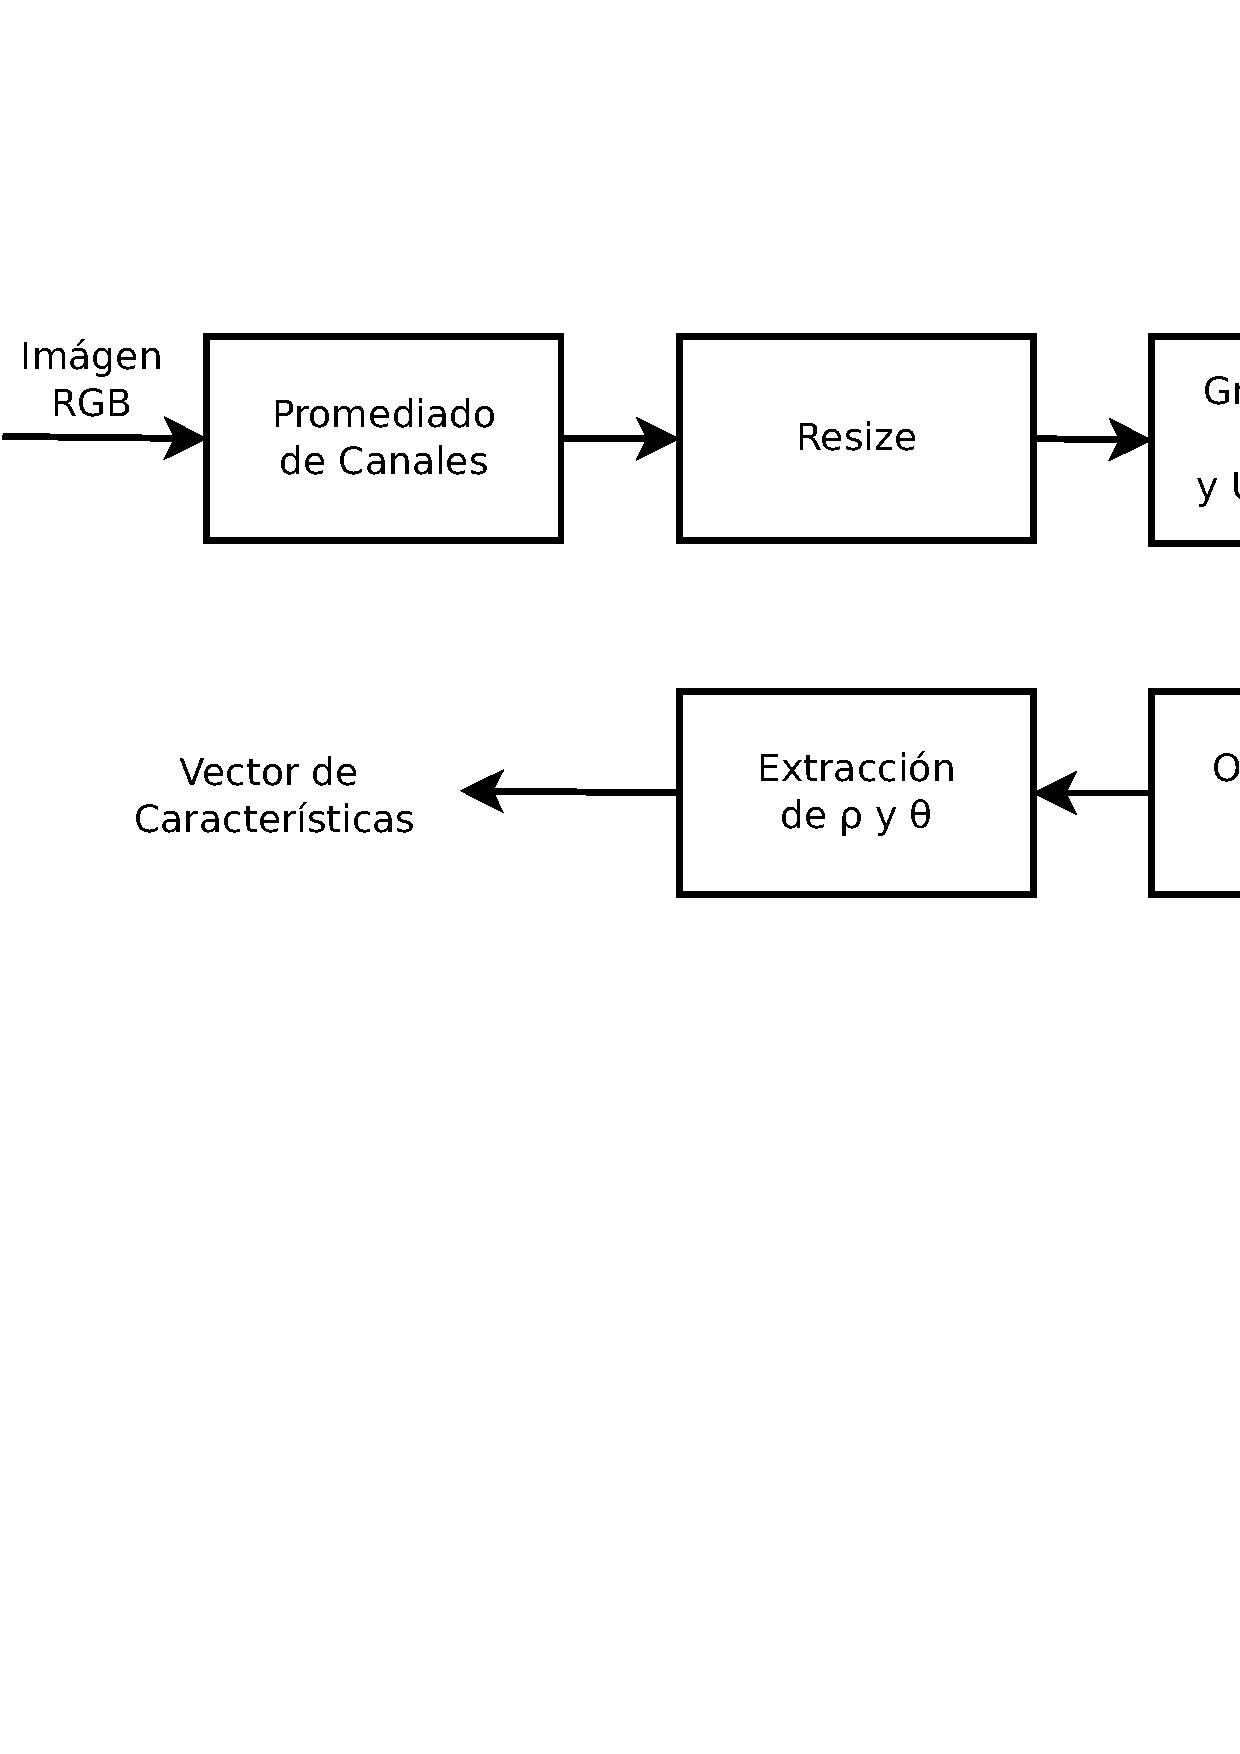
\includegraphics[scale=0.25]{../diagramas/procesohough} 
\caption{"Proceso de la imagen mediante el método por T. de Hough"}
\label{procesohough}
\end{figure}
%%%%%%%%%%%%%%%%%%%%%%%%%%%%%%%%%%%%%%%%%%%%%%%%%%%%%%%%%%%%%%%%%%%%%%%%%%%%%%%%%%%%%%%%%%
\subsection*{Método estadístico}
acá describir el método que hizo mauro..histogramas y demás....
%%%%%%%%%%%%%%%%%%%%%%%%%%%%%%%%%%%%%%%%%%%%%%%%%%%%%%%%%%%%%%%%%%%%%%%%%%%%%%%%%%
\section{Experimentos y resultados}
Para las pruebas se procedió a evaluar el desempeño de ambos métodos, en primera instancia por separados y luego, conjuntamente.
%%%%%%%%%%%%%%%%%%%%%%%%%%%%%%%%%%%%%%%%%%%%%%%%%%%%%%%%%%%%%%%%%%%%%%%%%%%%%%%%%%
\subsection{Descripción de la Base de datos de imágenes}
Se trabajó con imágenes que fueron adquiridas en la ciudad de Santa Fe, mediante un Dispositivo Móvil con una resolución de 640x480 pixels. Se construyo una base de datos de las mismas sobre un total de cinco edificios, tomando trece realizaciones de cada uno de ellos (diez con el propósito de usarlas como prototipo y tres para las prueba con los algoritmos). Cabe aclarar que cada conjunto de imágenes de los cinco edificios fueron tomadas en condiciones ambientales similares y con la cámara en la misma posición respecto del objetivo. \resalt{arreglar esto}.
%%%%%%%%%%%%%%%%%%%%%%%%%%%%%%%%%%%%%%%%%%%%%%%%%%%%%%%%%%%%%%%%%%%%%%%%%%%%%%%%%%
\subsection{Vectores característicos y prototipos}
Sobre diez de las trece imágenes de cada edificio, se aplicó el método de al Transformada de Hough citado en este artículo, obteniéndose diez vectores representativos (uno por cada imagen) y se procedió a promediar dichos vectores dando como resultado un prototipo por cada edifico. De la misma manera se realizó el mismo proceso, con el método estadístico descripto también en este documento.
%%%%%%%%%%%%%%%%%%%%%%%%%%%%%%%%%%%%%%%%%%%%%%%%%%%%%%%%%%%%%%%%%%%%%%%%%%%%%%%%%%
\subsection{Descripción de las pruebas}
Por cada método se calculo el MSE o error cuadratico medio definido en \ref{mse} entre los cinco prototipos y las quince imágenes de pruebas, para finalmente obtener la tasa de reconocimiento mediante \ref{tasareconocimiento}
\begin{equation}
MSE=\ldots \label{mse}
\end{equation}
\begin{equation}
\% reconocimiento = \frac{\# aciertos}{15} \label{tasareconocimiento}
\end{equation}
%
%
% %%%%%%%%%%%%%%%%%%%%%%%%%%%%%%%%%%%%%%%%%%%%%%%%%%%%%%%%%%%%%%%%%%%%%%%%%%%%%%
%
%
\subsection{Tablas}
\begin{tabular}{cc}
\hline columna1 & columna2 \\ 
\hline  &  \\ 
\hline 
\end{tabular} 
%
%
% %%%%%%%%%%%%%%%%%%%%%%%%%%%%%%%%%%%%%%%%%%%%%%%%%%%%%%%%%%%%%%%%%%%%%%%%%%%%%%
%
%
\subsection{Discusión}
blablabla
%
%
% %%%%%%%%%%%%%%%%%%%%%%%%%%%%%%%%%%%%%%%%%%%%%%%%%%%%%%%%%%%%%%%%%%%%%%%%%%%%%%
%
%
\section{Conclusiones}
blablabla
%
%
% %%%%%%%%%%%%%%%%%%%%%%%%%%%%%%%%%%%%%%%%%%%%%%%%%%%%%%%%%%%%%%%%%%%%%%%%%%%%%%
%
%
\section{Trabajos futuros}
A partir del diseño aquí presentado, seguiremos investigando esta técnica con las siguientes
posibilidades:
\begin{itemize}
\item blablabla
\end{itemize}

\nocite{*}
\bibliographystyle{tfmpd}
\bibliography{tfmpd}
\end{document}

